%-*- coding:utf-8 -*-

\section{偏微分方程式の初期値問題}

\begin{frame}[t]{一次元拡散方程式(放物型)}
  \begin{itemize}
  \item 一次元拡散方程式: $u=u(x,t)$, $q=q(x,t)$
    \[
    \frac{\partial u}{\partial t} - D \frac{\partial^2 u}{\partial x^2} = q
    \]
    \begin{itemize}
    \item 初期条件: $u(x,0) = f(x)$
    \item 境界条件: $u(0,t) = u(1,t) = 0$
    \end{itemize}
  \item 時間$t$と位置$x$に関して離散化
    \begin{align*}
      & u_j^n = u(x_j, t_n) \\
      & q_j^n = q(x_j, t_n) \\
      & t_0 = 0, t_1=\Delta t, t_2=2 \Delta t, \cdots, t_n=n \Delta t, \cdots \\
      & x_0 = 0, x_1=\Delta x, x_2=2 \Delta x, \cdots, x_N=N \Delta x = 1 \qquad (\Delta x = 1/N)
    \end{align*}
  \end{itemize}
\end{frame}

\begin{frame}[t]{有限差分法}
  \begin{itemize}
  \item $t$に関して前進差分を考える
    \[
    \frac{\partial u}{\partial t} \Big|_{(j \Delta x, n \Delta t)} = \frac{u_j^{n+1} - u_j^n}{\Delta t} + {\cal O}(\Delta t)
    \]
  \item $x$に関しては中心差分を考える
    \[
    \frac{\partial^2 u}{\partial x^2} \Big|_{(j \Delta x, n \Delta t)} = \frac{u_{j+1}^{n} - 2 u_{j}^{n} + u_{j-1}^{n}}{\Delta x^2} + {\cal O}(\Delta x^2)
    \]
  \item 拡散方程式に代入して整理すると
    \[
    u_{j}^{n+1} = u_{j}^{n} + r (u_{j+1}^{n} - 2 u_{j}^{n} + u_{j-1}^{n}) + \Delta t q_{j}^{n} \qquad (r = D\frac{\Delta t}{\Delta x^2})
    \]
  \item FTCS (Forward-Time Centered Space)法
  \end{itemize}
\end{frame}

\begin{frame}[t]{FTCS法}
  \begin{itemize}
  \item $O(\Delta t) + O(\Delta x^2)$の陽解法
    \begin{center}
      \resizebox{0.4\textwidth}{!}{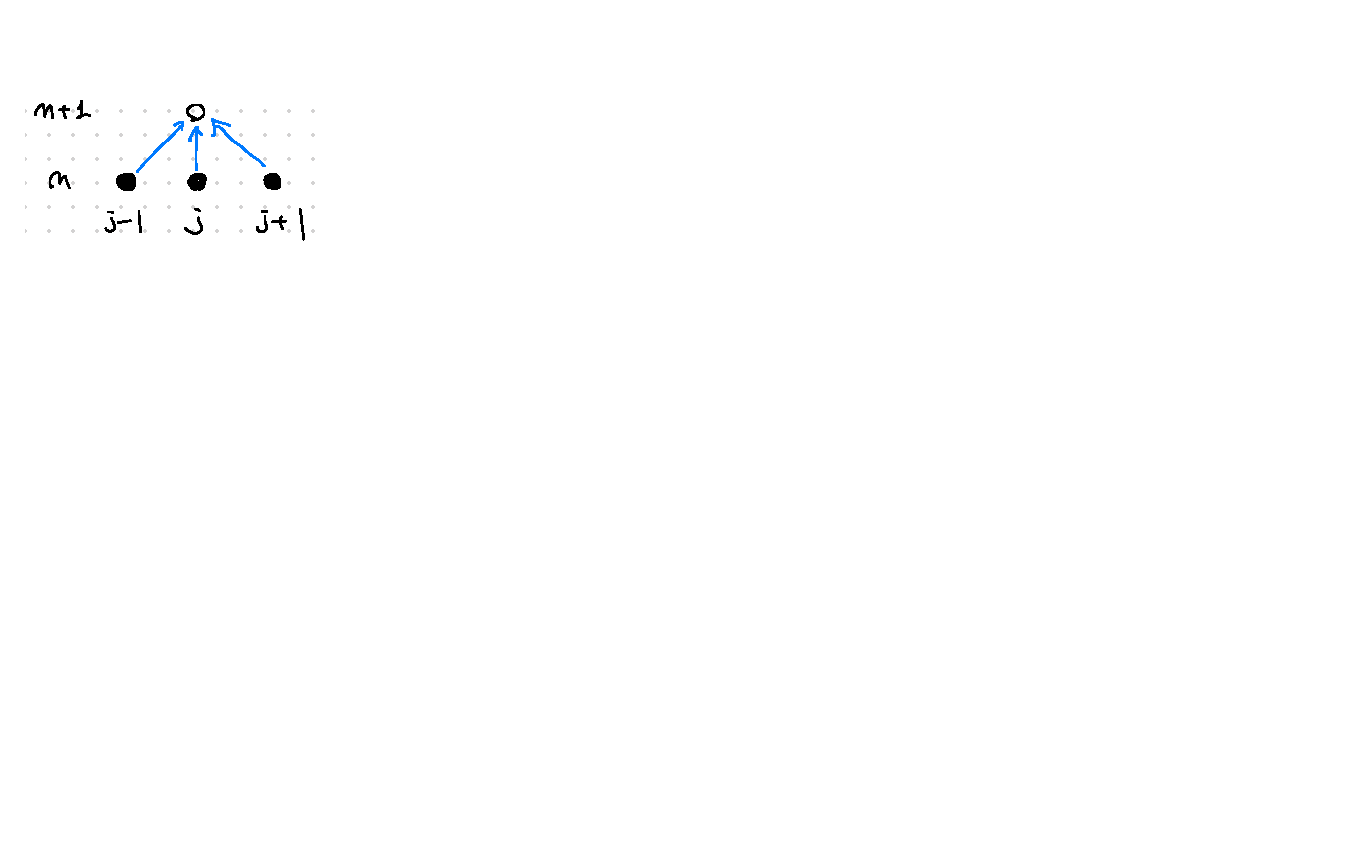
\includegraphics{image/ftcs-1.pdf}}
    \end{center}
  \item 初期条件
    \[
    u_j^0 = f(j\Delta x) \ \ (j=0,1,\cdots,N)
    \]
  \item 境界条件
    \[
    u_0^n = u_N^n = 0 \ \ (n=0,1,2,\cdots)
    \]
  \end{itemize}
\end{frame}

\begin{frame}[t]{有限差分法の安定性}
  \begin{itemize}
  \item (陽的)有限差分法においては、$\Delta t$、$\Delta x$は小さければ小さいほどよいというわけではない
  \item 一次元拡散方程式の場合
    \begin{align*}
      \begin{cases}
        r \le 1/2 & \text{安定} \\
        r > 1/2 & \text{\color{red}不安定}
      \end{cases}
    \end{align*}
  \item $\Delta x$を半分にしたら、$\Delta t$は1/4にしなければならない

    $\Rightarrow$ 計算量は8倍
  \end{itemize}
\end{frame}

\begin{frame}[t]{一次元波動方程式(双極型)}
  \begin{itemize}
  \item 一次元波動方程式
    \[
    \frac{\partial^2 u}{\partial t^2} = c^2 \frac{\partial^2 u}{\partial x^2} \qquad u(x,0)=f(x), \frac{\partial u}{\partial t} (x,0) = g(x)
    \]
  \item $t$に関する中心差分
    \[
    \frac{\partial^2 u}{\partial t^2} \Big|_{(j \Delta x, n \Delta t)} = \frac{u_{j}^{n+1} - 2 u_{j}^{n} + u_{j}^{n-1}}{\Delta t^2} + {\cal O}(\Delta t^2)
    \]
  \item 代入して整理すると
    \[
    u_{j}^{n+1} = 2u_{j}^{n} - u_{j}^{n-1} + \alpha^2 (u_{j+1}^{n} - 2 u_{j}^{n} + u_{j-1}^{n}) \qquad (\alpha = c\frac{\Delta t}{\Delta x})
    \]
  \end{itemize}
\end{frame}

\begin{frame}[t]{波動方程式に対するFTCS法}
  \begin{itemize}
  \item $O(\Delta t^2) + O(\Delta x^2)$の陽解法
    \begin{center}
      \resizebox{0.4\textwidth}{!}{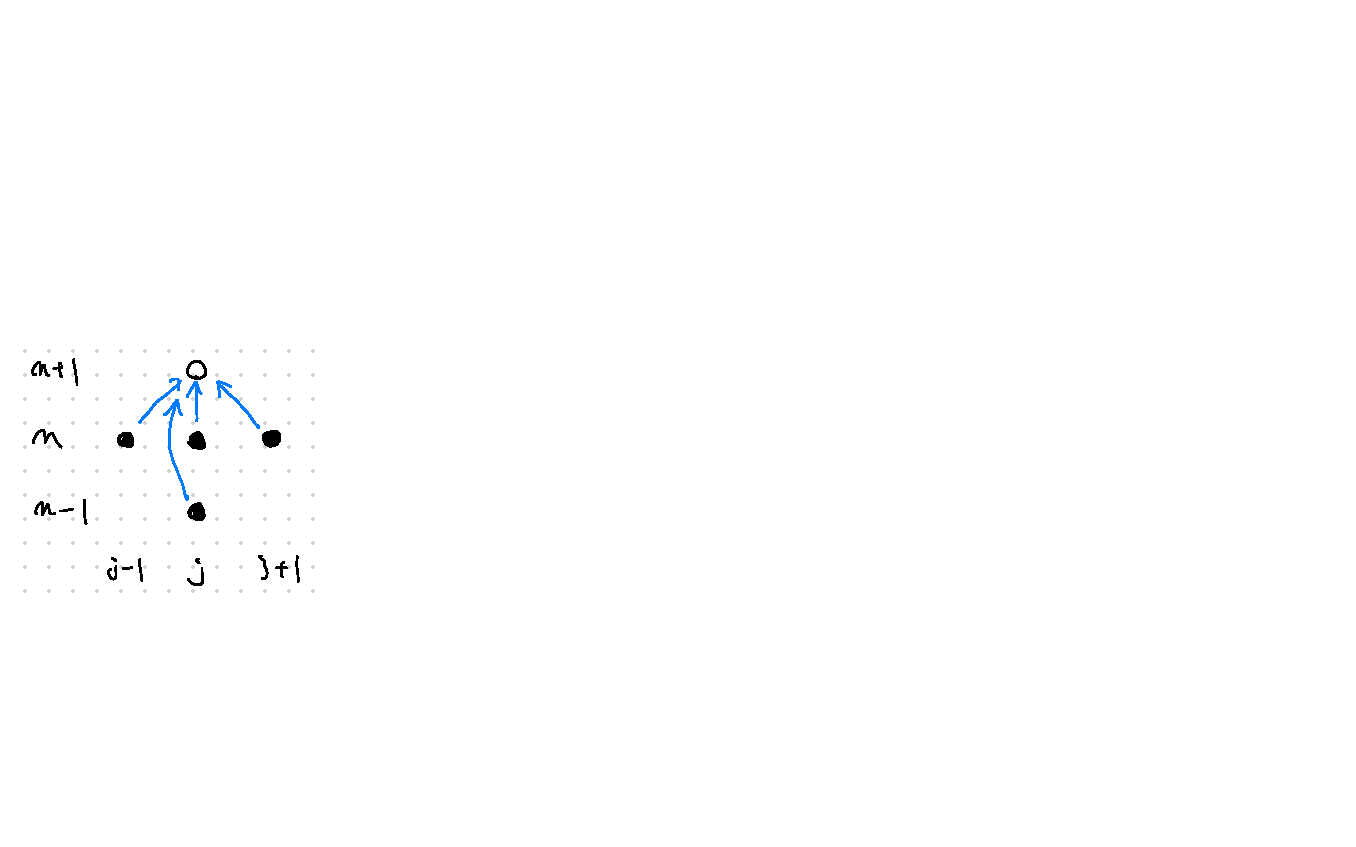
\includegraphics{image/ftcs-2.pdf}}
    \end{center}
  \item 初期条件
    \[
    u_j^0 = f(j\Delta x) \ \ (j=0,1,\cdots,N)
    \]
    初期速度については$n=0$に関する中心差分を考えて
    \[
    \frac{u_j^1 - u_j^{-1}}{2 \Delta t} = g_j \ \ \Rightarrow \ \ u_j^1 = u_j^0 + \Delta t g_j + \frac{\alpha^2}{2} (u_{j+1}^{n} - 2 u_{j}^{n} + u_{j-1}^{n})
    \]
  \end{itemize}
\end{frame}

\begin{frame}[t]{時間に依存するシュレディンガー方程式}
  \begin{itemize}
  \item 時間に依存するシュレディンガー方程式
    \[
    i \hbar \frac{\partial \Psi}{\partial t}(x,t) = H(x,t) \Psi(x,t) = \Big[ - \frac{\hbar^2}{2m} \frac{\partial^2}{\partial x^2} + V(x,t) \Big] \Psi(x,t)
    \]
    \begin{itemize}
    \item 波動関数のノルム $\displaystyle \int | \Psi(x,t) |^2 \, dx$ は保存
    \item $V(x,t)$が時間$t$に依存しない場合、エネルギーの期待値は保存
      \[
      \langle H \rangle = \frac{\displaystyle \int \Psi^* H \Psi \, dx}{\displaystyle \int | \Psi |^2 \, dx}
      \]
    \end{itemize}
  \item 以下では無次元化して$\hbar = m = 1$とおく
  \end{itemize}
\end{frame}

\begin{frame}[t]{時間に依存するシュレディンガー方程式}
  \begin{itemize}
  \item シュレディンガー方程式の形式解 ($V$が時間に依存しない場合)
    \[
    \Psi(x,t) = e^{-i H t} \Psi(x,0)
    \]
  \item $t$に関して前進差分
    \begin{align*}
      e^{-i H t} &= [e^{-i H \Delta t}]^M \approx [1 - i H \Delta t]^M \qquad (\Delta t = t / M) \\
      \Psi^{n+1} &= (1 -  i \Delta t H) \Psi^{n}
    \end{align*}
  \item $H$は対称(エルミート)行列 $\Rightarrow$ 時間発展演算子$e^{-i H \Delta t}$はユニタリー行列
  \item 差分近似$(1 -  i \Delta t H)$はユニタリーではない
    \begin{align*}
      & (e^{-i H \Delta t})^\dagger e^{-i H \Delta t} = e^{i H \Delta t} e^{-i H \Delta t} = 1 \\
      & (1 -  i \Delta t H)^\dagger (1 -  i \Delta t H) = (1 +  i \Delta t H) (1 -  i \Delta t H) = 1 + {\color{red} \Delta t^2 H^2}
    \end{align*}
  \end{itemize}
\end{frame}

\begin{frame}[t]{クランク・ニコルソン法}
  \begin{itemize}
  \item クランク・ニコルソン法
    \[
    \Psi^{n+1} = \frac{1 -  i \frac{\Delta t}{2} H}{1 +  i \frac{\Delta t}{2} H} \Psi^{n}
    \]
  \item (数値精度の範囲で)ユニタリー行列であるので、ノルムは保存
  \item $(1 +  i \frac{\Delta t}{2} H)^{-1}$を掛ける $\Rightarrow$ 連立一次方程式を解く必要がある
    \begin{itemize}
    \item まず、$\Psi = (1 - i \frac{\Delta t}{2} H) \Psi^n$ を計算
    \item 次に、$(1 +  i \frac{\Delta t}{2} H) \Psi^{n+1} = \Psi$ を解く(連立一次方程式)
    \end{itemize}
  \item 陰解法の一種
  \end{itemize}
\end{frame}

\begin{frame}[t]{陰解法}
  \begin{itemize}
  \item 時刻$t$関して後退差分を使う
    \[
    \frac{\partial u}{\partial t} \Big|_{(j \Delta x, n \Delta t)} = \frac{u_j^{n} - u_j^{n-1}}{\Delta t} + {\cal O}(\Delta t)
    \]
  \item $x$に関する中心差分と組み合わせ、$n \rightarrow n+1$と書き直すと
    \[
    u_{j}^{n+1} = u_{j}^{n} + r (u_{j+1}^{n+1} - 2 u_{j}^{n+1} + u_{j-1}^{n+1})
    \]
    $u^{n+1}$が両辺に現れる $\Rightarrow$ 陰解法
  \item $O(\Delta t) + O(\Delta x^2)$
  \item $r$の値によらず{\color{red}常に安定}
  \end{itemize}
\end{frame}

\begin{frame}[t]{クランク・ニコルソン法}
  \begin{itemize}
  \item さらに、時間方向にきざみ幅$\Delta t/2$の中心差分を使うと
    \[
    \frac{\partial u}{\partial t} \Big|_{(j \Delta x, n \Delta t)} = \frac{u_j^{n+\frac{1}{2}} - u_j^{n-\frac{1}{2}}}{\Delta t} + {\cal O}(\Delta t^2)
    \]
  \item $x$に関する中心差分と組み合わせ、$n \rightarrow n+\frac{1}{2}$し、さらに$u_j^{n+\frac{1}{2}}$を$(u_j^{n+1}+u_j^{n})/2$で近似すると
    \[
    u_{j}^{n+1} = u_{j}^{n} + \frac{r}{2} (u_{j+1}^{n+1} - 2 u_{j}^{n+1}  +u_{j-1}^{n+1} + u_{j+1}^{n} - 2 u_{j}^{n} + u_{j-1}^{n})
    \]
    あるいは
    \[
    u_{j}^{n+1} - \frac{r}{2} (u_{j+1}^{n+1} - 2 u_{j}^{n+1} + u_{j-1}^{n+1}) = u_{j}^{n} + \frac{r}{2} (u_{j+1}^{n} - 2 u_{j}^{n} + u_{j-1}^{n})
    \]
    $\Rightarrow$ クランク・ニコルソン法 [$O(\Delta t^2) + O(\Delta x^2)$]
  \end{itemize}
\end{frame}

%% \begin{frame}[t]{}
%%   \begin{itemize}
%%   \item
%%   \end{itemize}
%% \end{frame}
